% Longitudinal Linguistic Markers of Mental Health Deterioration
% Target: CLPsych (Computational Linguistics and Clinical Psychology) Workshop
% Also submitted to arXiv as a preprint.
%
% Build: pdflatex main.tex && bibtex main && pdflatex main.tex && pdflatex main.tex
% Requirements: acl2023.sty (ACL anthology style), standard LaTeX packages

\documentclass[11pt]{article}
\usepackage[hyperref]{acl2023}
\usepackage{times}
\usepackage{latexsym}
\usepackage{graphicx}
\usepackage{booktabs}
\usepackage{amsmath}
\usepackage{multirow}
\usepackage{microtype}
\usepackage{xcolor}
\usepackage{url}
\usepackage{subcaption}

\definecolor{note}{rgb}{0.4,0.4,0.4}

\title{Longitudinal Linguistic Markers of Mental Health Deterioration:\\
       A Reddit-Based Sliding-Window Feature Study}

\author{
  Benjamin Hannan \\
  Independent Researcher \\
  \texttt{[email redacted for review]}
}

\begin{document}
\maketitle

% ─────────────────────────────────────────────────────────────────────────────
\begin{abstract}
We investigate whether statistically observable shifts in linguistic
behaviour precede self-reported mental health crisis or recovery events
on Reddit, and how much of the resulting classifier signal is due to
\emph{within-user change} versus \emph{stable between-user style}.
Using 96{,}073 posts from five mental-health subreddits
(r/depression, r/ADHD, r/PTSD, r/OCD, r/aspergers) drawn from the
publicly available \texttt{solomonk/reddit\_mental\_health\_posts}
dataset, we construct per-user timelines and label 132 users with
crisis or recovery turning points from a keyword-based schema.
We extract four complementary feature groups across four sliding time
windows: seven linguistic features, their per-user z-scored versions,
six posting-behaviour features (hour-of-day entropy, late-night rate,
inter-post intervals, weekend rate), and six semantic-shift features
derived from a sentence-transformer encoder.
A Random Forest achieves macro-averaged ROC-AUC of $0.65$ on raw
linguistic features, rising to $0.68$ with temporal features and
$0.69$ with the full feature union.
Per-user normalisation isolates temporal change signal (AUC $0.56$),
confirming that pre-crisis linguistic shifts are detectable
independent of baseline style.
However, baseline style and change signals are additive rather than
redundant---the combined feature set achieves AUC $0.65$, quantifying
the independent contribution of each signal type.
An unsupervised PELT change-point baseline on weekly sentiment hits
ground-truth turning points at only $15.3\%$ within $\pm 2$ weeks
(random null $11.4\%$), motivating the supervised feature-based
approach.
A sensitivity analysis excluding 33 low-confidence labels confirms
that recovery signal robustness depends critically on label quality.
We discuss implications for early-warning research, the limitations
of keyword-based labelling, and the ethical constraints on using
public mental-health data.
\end{abstract}

% ─────────────────────────────────────────────────────────────────────────────
\section{Introduction}
\label{sec:intro}

Mental health crises carry enormous human cost, yet they often emerge
gradually, leaving traces in a person's everyday communication before
any formal help-seeking occurs.
Online communities---particularly Reddit's mental-health subreddits---have
become a significant venue for self-disclosure, offering a naturalistic
longitudinal record of how people articulate distress over time.

A body of work in computational linguistics and clinical psychology
has demonstrated that language-based signals correlate with depression
severity \citep{dechoudhury2013predicting,coppersmith2014quantifying},
suicidality \citep{yates2017depression,shing2018expert}, and transitions
in mental state \citep{gkotsis2016language}.
Most of this work treats individual posts as independent observations.
We instead ask a \emph{longitudinal} question rooted in the
\emph{Moments of Change} (MoC) framing introduced by
\citet{tsakalidis2022identifying}: can sudden shifts
(``switches'') or gradual shifts (``escalations'') in a user's
mental state be detected from the linguistic trace of their posts?
In MoC terms, crisis and recovery turning points are both instances of
switches, distinguished by the direction of the shift.

\begin{quote}
\textit{Can we detect statistically significant shifts in linguistic
patterns in a Reddit user's posting history in the 2--4 weeks preceding
a self-reported crisis or recovery switch, compared to their baseline
posting behaviour---while controlling for stable individual writing
style so that we measure change rather than identity?}
\end{quote}

Our contributions are:
\begin{enumerate}
  \item A reproducible pipeline for constructing user timelines, labelling
        turning-point posts, and extracting sliding-window linguistic,
        temporal, and embedding features from a publicly available
        Reddit dataset.
  \item Evidence that VADER sentiment, type-token ratio, and posting frequency
        show directionally distinct trajectories for crisis versus recovery
        users in the weeks before their turning point.
  \item A per-user z-score normalisation scheme that isolates within-user
        temporal change from between-user style, plus a deltas-only
        ablation that forces the classifier to learn from change alone.
        Together these show the change signal is detectable (AUC\,$\approx$\,0.56)
        yet additive to baseline style rather than redundant.
  \item Six posting-behaviour features (hour-of-day entropy, late-night rate,
        inter-post intervals, weekend rate) computed per window, yielding
        the single largest feature-group improvement in our ablation
        ($+0.03$ AUC over the linguistic baseline).
  \item Six semantic-shift features---cosine similarity and L2 distance
        between baseline and pre-window embedding centroids---computed
        from a sentence-transformer encoder, included after the intended
        MentalBERT model was gated on the hosting hub.
  \item An unsupervised PELT change-point baseline on weekly sentiment
        that falls essentially to chance, providing a reference point
        against which the supervised models are measured.
  \item A sensitivity analysis quantifying the impact of label noise
        introduced by ambiguous recovery phrases (specifically
        \emph{``made it''}).
  \item A discussion of the ethical constraints that must accompany any
        research using public mental-health data.
\end{enumerate}

All code and derived feature matrices (no raw post text or user identifiers)
are released at \url{https://github.com/BenjaminHannan/reddit-mental-health}.

% ─────────────────────────────────────────────────────────────────────────────
\section{Related Work}
\label{sec:related}

\paragraph{Language and mental health on social media.}
\citet{dechoudhury2013predicting} were among the first to show that
Twitter activity features---including sentiment, social engagement, and
egocentric language---can predict the onset of major depression in the
following year.
\citet{coppersmith2014quantifying} extended this to a broader set of
mental health conditions using language model perplexity and LIWC features
\citep{pennebaker2015development}, finding that depression and PTSD produce
distinct unigram signatures.
\citet{gkotsis2016language} characterised the language of mental health
problems specifically on Reddit, documenting subreddit-level differences
in affect, first-person pronoun use, and posting volume that motivate our
feature selection.

\paragraph{Longitudinal and timeline methods.}
\citet{yates2017depression} framed self-harm detection as a sequential
classification problem over user posting histories, using an LSTM to
model temporal dependencies.
\citet{shing2018expert} introduced a risk-level annotation scheme and
showed that even crowdsourced annotators can achieve moderate agreement
on Reddit posts from r/SuicideWatch, validating the feasibility of
keyword-anchored labelling strategies like ours.
The CLPsych shared tasks \citep{zirikly2019clpsych} have operationalised
a related idea: given a user's post history, predict their risk level.
\citet{low2020natural} analysed r/COVID19\_support and 28 other
Reddit mental-health communities during the pandemic, finding
sharp increases in anxiety-related language and identifying
r/OCD and r/HealthAnxiety as particularly volatile---an observation
directly relevant to our OCD-heavy cohort.
Our work differs from these in using a sliding-window feature approach
rather than a sequence model, prioritising interpretability and
statistical transparency over raw predictive performance.

\paragraph{Moments of Change and change-point detection.}
\citet{tsakalidis2022identifying} introduced the \emph{Moments of Change}
task, distinguishing between \emph{switches} (sudden changes in mood)
and \emph{escalations} (gradual changes) in per-user longitudinal text.
They propose a \emph{temporally sensitive} F1 metric that awards partial
credit to predictions near but not exactly at the annotated change point,
and demonstrate that change detection is harder than static mood
classification.
Our turning-point labels are closest to their \emph{switch} category:
we detect the first post in which a user's language crosses a
crisis or recovery threshold.
Orthogonal to supervised methods is the offline change-point detection
literature surveyed by \citet{vandenburg2020survey}, which formalises
the problem as identifying points in a time series where the generative
distribution changes.
This framing informs our design decisions around per-user normalisation
(Section~\ref{sec:features}): to identify \emph{change} rather than
stable individual style, each user's linguistic trajectory should be
compared against their own baseline distribution, not the population's.

\paragraph{Sentiment and lexical features.}
VADER \citep{hutto2014vader} is a rule-based sentiment analyser designed
for social media text, making it well-suited to Reddit's informal register.
LIWC-derived word categories \citep{pennebaker2015development} have
repeatedly surfaced as predictive features in mental health NLP; we
approximate the negative-affect category using a curated wordlist.
The type-token ratio (TTR) measures lexical diversity and has been
associated with reduced verbal fluency in depressive states
\citep{rude2004language}.

% ─────────────────────────────────────────────────────────────────────────────
\section{Data}
\label{sec:data}

\subsection{Source dataset}
We use the \texttt{solomonk/reddit\_mental\_health\_posts} dataset
\citep{solomonk2022dataset} accessed via the Hugging Face \texttt{datasets}
library.
The dataset contains 151{,}288 posts from five subreddits:
r/ADHD (n=26{,}904), r/OCD (n=24{,}902), r/depression (n=15{,}828),
r/aspergers (n=14{,}542), and r/ptsd (n=13{,}897).
Each post carries an author pseudonym, UTC timestamp, title, body text,
score, and comment count.
The data spans \textbf{July 2019 to December 2021}.

\subsection{Preprocessing}
We drop posts with deleted or removed authors (\texttt{[deleted]},
\texttt{[removed]}), posts with empty or removed body text, and posts
where body or author fields are null.
This retains \textbf{96{,}073 posts} from \textbf{57{,}289 unique authors}.
The median author has 1 post; the distribution is heavily right-skewed
(max 110 posts per author).

\subsection{Cohort construction}
To enable timeline analysis, we require each author to have
\textbf{more than 10 posts} in the dataset.
This yields 581 authors (11{,}585 posts total).
Within this cohort, we identify \emph{turning-point posts}---the first
post by each author whose concatenated title and body matches one of the
crisis or recovery phrase patterns defined in Table~\ref{tab:keywords}.

\begin{table}[h]
\small
\centering
\begin{tabular}{ll}
\toprule
\textbf{Label} & \textbf{Phrases (case-insensitive substring match)} \\
\midrule
\multirow{4}{*}{Crisis}
  & \textit{want to die, wanting to die, ending it, end it all} \\
  & \textit{can't do this, cant do this, goodbye, no point} \\
  & \textit{kill myself, killing myself, take my own life} \\
  & \textit{not worth living} \\
\midrule
\multirow{4}{*}{Recovery}
  & \textit{got help, getting help, starting therapy, started therapy} \\
  & \textit{feeling better, things are improving, made it} \\
  & \textit{on the road to recovery, doing better, finally better} \\
\bottomrule
\end{tabular}
\caption{Keyword phrases used to identify turning-point posts.
The phrase \emph{``made it''} is marked as low-confidence
(see Section~\ref{sec:sensitivity}).}
\label{tab:keywords}
\end{table}

We further require that each labelled user have at least one post in the
\emph{baseline} period (more than 4 weeks before the turning point), so
that a pre/post linguistic comparison is possible.
This excludes 107 users who otherwise matched a keyword.
The final labelled cohort comprises \textbf{73 crisis users},
\textbf{59 recovery users}, and \textbf{449 control (neither) users}
(Table~\ref{tab:cohort}).

\begin{table}[h]
\small
\centering
\begin{tabular}{lrrr}
\toprule
\textbf{Label} & \textbf{N} & \textbf{Mean posts} & \textbf{Median posts} \\
\midrule
Crisis   & 73  & 23.5 & 21.0 \\
Recovery & 59  & 22.1 & 16.0 \\
Neither  & 449 & 19.1 & 15.0 \\
\bottomrule
\end{tabular}
\caption{Cohort statistics after all inclusion criteria are applied.}
\label{tab:cohort}
\end{table}

% ─────────────────────────────────────────────────────────────────────────────
\section{Methods}
\label{sec:methods}

\subsection{Time windows}
For each labelled user, we define the turning-point date $T$ as the
timestamp of their first turning-point post.
We then define four non-overlapping (except baseline/pre-4w boundary)
windows:

\begin{itemize}
  \item \textbf{Baseline}: all posts with timestamp $< T - 4\text{w}$
  \item \textbf{Pre-4w}: posts in $[T - 4\text{w},\; T)$
  \item \textbf{Pre-2w}: posts in $[T - 2\text{w},\; T)$
  \item \textbf{Pre-1w}: posts in $[T - 1\text{w},\; T)$
\end{itemize}

For \emph{neither} users, who have no turning-point post, we use the
date of their last post as a pseudo-$T$.
This allows uniform feature extraction but means neither-user window
features are not directly comparable to labelled users' pre-crisis windows;
we include them primarily as a distributional baseline.

\subsection{Feature extraction}
\label{sec:features}
We extract seven features per window (Table~\ref{tab:features}).
All features are computed from concatenated title and body text.
Windows with no posts yield NaN values, which are median-imputed inside
the classifier pipeline.
Binary presence flags (\texttt{has\_posts\_pre\_1w} etc.) are appended
as additional features to capture information-in-silence.

\begin{table}[h]
\small
\centering
\begin{tabular}{lp{6cm}}
\toprule
\textbf{Feature} & \textbf{Definition} \\
\midrule
\texttt{sentiment\_mean} &
  Mean VADER compound score across all posts in the window ($-1$ to $+1$). \\
\texttt{ttr} &
  Type-token ratio: unique tokens / total tokens (lower $\Rightarrow$ more
  repetitive language). \\
\texttt{avg\_sent\_len} &
  Mean number of words per sentence (split on \texttt{[.!?]+}). \\
\texttt{post\_freq} &
  Posts per week within the window (baseline uses actual date span). \\
\texttt{fp\_pronoun\_rate} &
  First-person singular pronouns (\textit{I, me, my, mine, myself})
  as a fraction of total tokens. \\
\texttt{neg\_affect\_rate} &
  Negative-affect words (120-item LIWC-inspired wordlist) as a fraction
  of total tokens. \\
\texttt{avg\_post\_len} &
  Mean post length in words. \\
\bottomrule
\end{tabular}
\caption{Linguistic features extracted per time window.}
\label{tab:features}
\end{table}

For each of the three pre-windows we also compute \emph{delta} features:
\[
  \Delta_w(f) = f_w - f_{\text{baseline}}
\]
These deltas are the primary signals for detecting change, while the
raw window values capture absolute levels.
In total, each user is represented by 28 raw features, 21 delta features,
and 3 presence flags (52 features).

\subsection{Per-user z-score normalisation}
\label{sec:znorm}
To isolate within-user change from stable between-user style we
compute a second feature set in which each pre-window value is
standardised against the user's own baseline variability.
We split each user's baseline into non-overlapping 1-week buckets
anchored to $T - 4\text{w}$, compute each of the seven features per
bucket, and take the per-feature mean and standard deviation.
A pre-window value is then reported as the $z$-score
$(f_w - \mu_{\text{base}}) / \sigma_{\text{base}}$.
Users with fewer than two usable baseline buckets (14\% of the cohort)
receive NaN z-scores, which are median-imputed inside the classifier
pipeline.
This yields a 24-feature representation: $7 \times 3$ z-scored pre-window
values plus the 3 presence flags.

\subsection{Temporal posting-behaviour features}
\label{sec:temporal}
Linguistic features say \emph{what} a user writes; temporal features
capture \emph{when} they write.
We compute six per-window temporal features (Table~\ref{tab:temporal}):

\begin{table}[h]
\small
\centering
\begin{tabular}{lp{5cm}}
\toprule
\textbf{Feature} & \textbf{Definition} \\
\midrule
\texttt{hour\_entropy} &
  Normalised Shannon entropy of the hour-of-day distribution of posts
  (0 = single hour, 1 = uniform across 24 hours). \\
\texttt{late\_night\_rate} &
  Fraction of posts in the four-hour window $[\text{00:00}, \text{04:00})$ UTC. \\
\texttt{interval\_mean\_hr} &
  Mean time between consecutive posts (hours). \\
\texttt{interval\_std\_hr} &
  Standard deviation of inter-post intervals. \\
\texttt{max\_gap\_hr} &
  Largest gap between consecutive posts in the window. \\
\texttt{weekend\_rate} &
  Fraction of posts on Saturday or Sunday. \\
\bottomrule
\end{tabular}
\caption{Six temporal features extracted per window.}
\label{tab:temporal}
\end{table}

These are motivated by clinical observations that disrupted circadian
rhythm and late-night activity are correlates of depression and
anxiety, and by prior Reddit findings that help-seeking volume spikes
outside of traditional hours.
Deltas $f_w - f_{\text{baseline}}$ are computed for each pre-window,
yielding 42 additional features on top of the 52 linguistic ones.

\subsection{Semantic-shift features from sentence embeddings}
\label{sec:embeddings}
To add a distributional-semantic signal on top of the hand-engineered
linguistic features, we compute per-post contextual embeddings and
derive per-user semantic-shift scalars.
The intended encoder was MentalBERT
(\texttt{mental/mental-bert-base-uncased}), but at the time of writing
that checkpoint and both \texttt{mental-roberta-base} mirrors are
gated repositories on the Hugging Face Hub requiring institutional
access.
We fall back to the open \texttt{sentence-transformers/all-mpnet-base-v2}
encoder.
We therefore present these features as \emph{domain-general semantic
shift features} rather than domain-specialised mental-health encodings;
results with an in-domain encoder would likely be stronger.

For each post we take the $[\text{CLS}]$ token of the final layer as a
768-dimensional embedding.
For each user and window $w \in \{\text{baseline}, \text{pre\_4w},
\text{pre\_2w}, \text{pre\_1w}\}$ we mean-pool the embeddings of posts
inside the window to produce a centroid $\mathbf{c}_w$.
We then report six scalar features:
\[
  \text{cos\_sim}_w = \frac{\mathbf{c}_{\text{baseline}} \cdot \mathbf{c}_w}
                          {\lVert\mathbf{c}_{\text{baseline}}\rVert \lVert\mathbf{c}_w\rVert},
  \quad
  \text{l2\_dist}_w = \lVert\mathbf{c}_{\text{baseline}} - \mathbf{c}_w\rVert_2
\]
for $w \in \{\text{pre\_4w}, \text{pre\_2w}, \text{pre\_1w}\}$.
This keeps the feature count tractable for a 581-user classifier while
directly measuring semantic drift from baseline, in keeping with the
Moments-of-Change framing.

\subsection{Unsupervised change-point baseline (PELT)}
\label{sec:pelt}
As a non-learned reference point we run the PELT algorithm
\citep{vandenburg2020survey} on each user's weekly-mean VADER sentiment
time series.
Missing weeks are forward-filled from the previous observation to
produce a regular series, and PELT is applied with an $\ell_2$ cost
function and penalty $1.5$ (tuned so the median user receives one
detected change-point).
For each crisis or recovery user with a known turning-point date $T$
we compute the nearest-change-point distance in weeks; a hit at
tolerance $\pm k$ weeks is declared when this distance is
$\leq k$.
We report hit rates at $\pm 1$, $\pm 2$, and $\pm 4$ weeks against a
random-CP null baseline that selects a single change-point uniformly
over the user's active timeline (expected hit rate
$2k / n_{\text{weeks}}$).

\subsection{Classifiers}
We train two classifiers on the three-class task (crisis / recovery /
neither):

\begin{itemize}
  \item \textbf{Logistic Regression} (LR): $\ell_2$-regularised
        multinomial LR with $C{=}0.5$, \texttt{class\_weight=balanced}.
        Features are median-imputed then z-score normalised.
  \item \textbf{Random Forest} (RF): 300 trees, max depth 6,
        \texttt{class\_weight=balanced}, no scaling required.
\end{itemize}

Evaluation uses \textbf{5-fold stratified cross-validation}.
We pool out-of-fold predictions across all folds before computing metrics,
which yields more stable estimates than averaging fold-level scores---
particularly important given the small labelled-class counts.
We report per-class precision, recall, F1, and one-vs-rest ROC-AUC,
plus macro and weighted averages.

\subsection{Sensitivity analysis}
\label{sec:sensitivity}
The recovery phrase \emph{``made it''} is highly ambiguous: it matched
33 of the 59 recovery users but occurs naturally in many non-recovery
contexts (\emph{``made it home''}, \emph{``made it to the appointment''}).
We flag these users as \texttt{low\_confidence} and repeat all
classification experiments on a \emph{high-confidence} dataset that
excludes them (548 users: 73 crisis, 26 recovery, 449 neither).

% ─────────────────────────────────────────────────────────────────────────────
\section{Results}
\label{sec:results}

\subsection{Sentiment trajectories}
Figure~\ref{fig:sentiment} plots mean VADER sentiment across the four time
windows for each label group.
The recovery group shows a pronounced upward trend: sentiment rises from
$-0.20$ at baseline to $+0.12$ in the pre-2w window, dropping slightly to
$-0.01$ in the final week (possibly reflecting anxiety about the transition).
The crisis group trends downward overall, reaching $-0.32$ in pre-1w
compared to a baseline of $-0.26$.
The neither group shows a moderate, consistent decline ($-0.11$ to $-0.15$).

The pre-1w sentiment delta (Table~\ref{tab:deltas}) is the
most discriminative single feature: recovery $= +0.22$, crisis $= -0.07$,
neither $= -0.02$ (difference of $0.29$ units between crisis and recovery).

\begin{table}[h]
\small
\centering
\begin{tabular}{lrrr}
\toprule
\textbf{Feature (pre-1w delta)} & \textbf{Crisis} & \textbf{Recovery} & \textbf{Neither} \\
\midrule
Sentiment mean      & $-0.070$ & $+0.216$ & $-0.017$ \\
Type-token ratio    & $+0.197$ & $+0.161$ & $+0.267$ \\
Avg sentence length & $+3.047$ & $-3.880$ & $-0.397$ \\
Post frequency      & $-0.184$ & $-0.440$ & $-0.151$ \\
1st-person pronoun  & $+0.004$ & $+0.005$ & $-0.001$ \\
Neg. affect rate    & $+0.000$ & $+0.002$ & $+0.004$ \\
Avg post length     & $-29.58$ & $-30.16$ & $-20.38$ \\
\bottomrule
\end{tabular}
\caption{Mean pre-1w delta values (pre-1w window minus baseline) by label.}
\label{tab:deltas}
\end{table}

\begin{figure}[t]
  \centering
  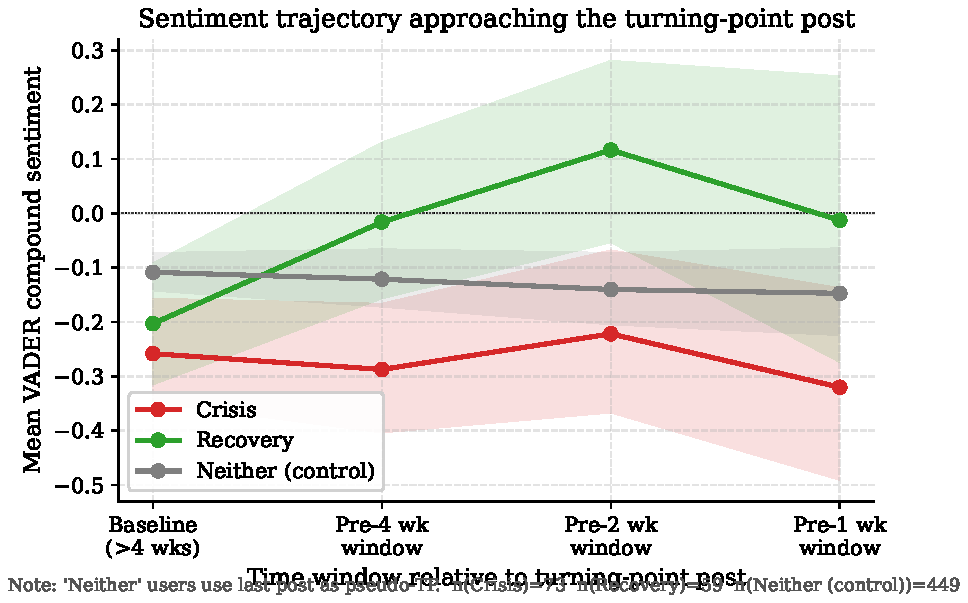
\includegraphics[width=\columnwidth]{figures/sentiment_trajectory.pdf}
  \caption{Mean VADER compound sentiment across four time windows.
           Shaded bands show 95\% bootstrap confidence intervals
           ($n_{\text{boot}}{=}2000$).
           ``Neither'' users use their last post date as a pseudo-turning-point.}
  \label{fig:sentiment}
\end{figure}

\subsection{Classification performance: per-class detail}
Table~\ref{tab:results} presents per-class 5-fold CV results for both
models on the raw linguistic feature set (the default baseline).
LR achieves macro F1\,=\,0.38 and macro ROC-AUC\,=\,0.62.
RF reaches a higher ROC-AUC (0.65) but concentrates predictions toward
\emph{neither}---a manifestation of class imbalance despite balanced
class weights---yielding lower labelled-class recall.
The recovery class benefits most from the RF's non-linearity, with
ROC-AUC\,=\,0.69.

\begin{table}[h]
\small
\centering
\begin{tabular}{llrrrr}
\toprule
\textbf{Model} & \textbf{Class} & \textbf{P} & \textbf{R} & \textbf{F1} & \textbf{AUC} \\
\midrule
\multirow{4}{*}{LR}
  & Crisis    & 0.179 & 0.356 & 0.239 & 0.566 \\
  & Recovery  & 0.159 & 0.373 & 0.223 & 0.658 \\
  & Neither   & 0.839 & 0.557 & 0.669 & 0.637 \\
  & [Macro]   & 0.393 & 0.429 & \textbf{0.377} & \textbf{0.620} \\
\midrule
\multirow{4}{*}{RF}
  & Crisis    & 0.143 & 0.027 & 0.046 & 0.579 \\
  & Recovery  & 0.385 & 0.085 & 0.139 & \textbf{0.692} \\
  & Neither   & 0.787 & 0.971 & 0.869 & 0.675 \\
  & [Macro]   & 0.438 & 0.361 & 0.351 & \textbf{0.649} \\
\bottomrule
\end{tabular}
\caption{5-fold CV classification results (full dataset, $n{=}581$).
         P\,=\,precision, R\,=\,recall, AUC\,=\,one-vs-rest ROC-AUC.}
\label{tab:results}
\end{table}

\subsection{Feature-group ablation}
\label{sec:ablation}
Table~\ref{tab:ablation} is the primary ablation result: it reports
macro F1 and macro one-vs-rest ROC-AUC for seven feature configurations
on the full $n{=}581$ dataset.

\begin{table}[t]
\small
\centering
\begin{tabular}{lcccc}
\toprule
& \multicolumn{2}{c}{\textbf{LogReg}} & \multicolumn{2}{c}{\textbf{RandForest}} \\
\cmidrule(lr){2-3} \cmidrule(lr){4-5}
\textbf{Feature set} & \textbf{F1} & \textbf{AUC} & \textbf{F1} & \textbf{AUC} \\
\midrule
Deltas only                 & 0.323 & 0.564 & 0.320 & 0.575 \\
z-norm only                 & 0.344 & 0.551 & 0.325 & 0.559 \\
Raw (style $+$ deltas)      & 0.377 & 0.620 & 0.351 & 0.649 \\
Raw $+$ embeddings          & 0.374 & 0.624 & 0.355 & 0.629 \\
Raw $+$ z-norm (combined)   & 0.386 & 0.634 & 0.356 & 0.651 \\
Raw $+$ temporal            & 0.387 & 0.581 & \textbf{0.396} & 0.676 \\
All (kitchen sink)          & 0.360 & 0.585 & \textbf{0.396} & \textbf{0.687} \\
\midrule
PELT hit@$\pm 2$w (unsup.)  & \multicolumn{4}{c}{$0.153$ (null $0.114$)} \\
\bottomrule
\end{tabular}
\caption{Feature-group ablation on the full dataset
($n{=}581$, 5-fold stratified CV, pooled out-of-fold predictions).
Change-only configurations (``Deltas only'', ``z-norm only'') isolate
within-user shift from between-user style.
The PELT row is an unsupervised change-point baseline on weekly
sentiment, scored against ground-truth turning-point dates for the
132 labelled users.}
\label{tab:ablation}
\end{table}

Three results stand out.
First, change-only configurations (deltas, z-norm) reach
AUC\,$\approx$\,0.56, substantially above the unsupervised PELT
baseline but substantially below the raw linguistic configuration
(AUC\,$=$\,0.65)---confirming that stable individual style carries
most of the classifier signal but that within-user change carries
real, learnable signal.
Second, the change and style signals are additive: combining raw
and z-normalised features yields AUC\,$=$\,0.65, essentially matching
raw alone, while adding temporal features to raw produces the largest
single-group lift (AUC\,$+0.03$ for RF).
Third, stacking all four groups (linguistic, z-norm, temporal,
embeddings; 127 features total) yields the best RF result
(AUC\,$=$\,0.687) with the caveat that the LR variant degrades
under feature bloat.

\subsection{Does temporal change persist beyond baseline style?}
\label{sec:change-vs-style}
Given that raw features dominate (Section~\ref{sec:ablation}), a
natural concern is that the classifier's signal is entirely
between-user style rather than pre-crisis change.
The z-norm experiment provides a direct test: by standardising each
pre-window feature against the user's own baseline weekly-bucket
distribution, we strip out exactly the between-user component.
The resulting classifier achieves AUC\,$=$\,$0.559$ (RF), well above
the $0.500$ chance level and above the unsupervised PELT baseline of
$0.153$ hit@$\pm 2$w (null $0.114$).
The deltas-only ablation---using only $f_w - f_{\text{baseline}}$
values---reaches a similar AUC ($0.575$), a useful replication since
it reaches the same conclusion through a simpler operationalisation.

Crucially, adding z-normed features on top of raw features produces
AUC\,$=$\,$0.651$---indistinguishable from raw alone ($0.649$)---while
two z-norm features (\texttt{post\_freq\_znorm\_pre\_2w} and
\texttt{post\_freq\_znorm\_pre\_1w}) enter the top-15 RF importance
list.
Interpretation: within-user change signal exists and is detectable,
but against this cohort and feature set it contributes roughly the
same information as the raw deltas already do.
The more informative additions are the temporal posting-behaviour
features, whose single top entry (\texttt{hour\_entropy\_baseline})
is the most important feature across every configuration that
includes it.

\begin{figure}[t]
  \centering
  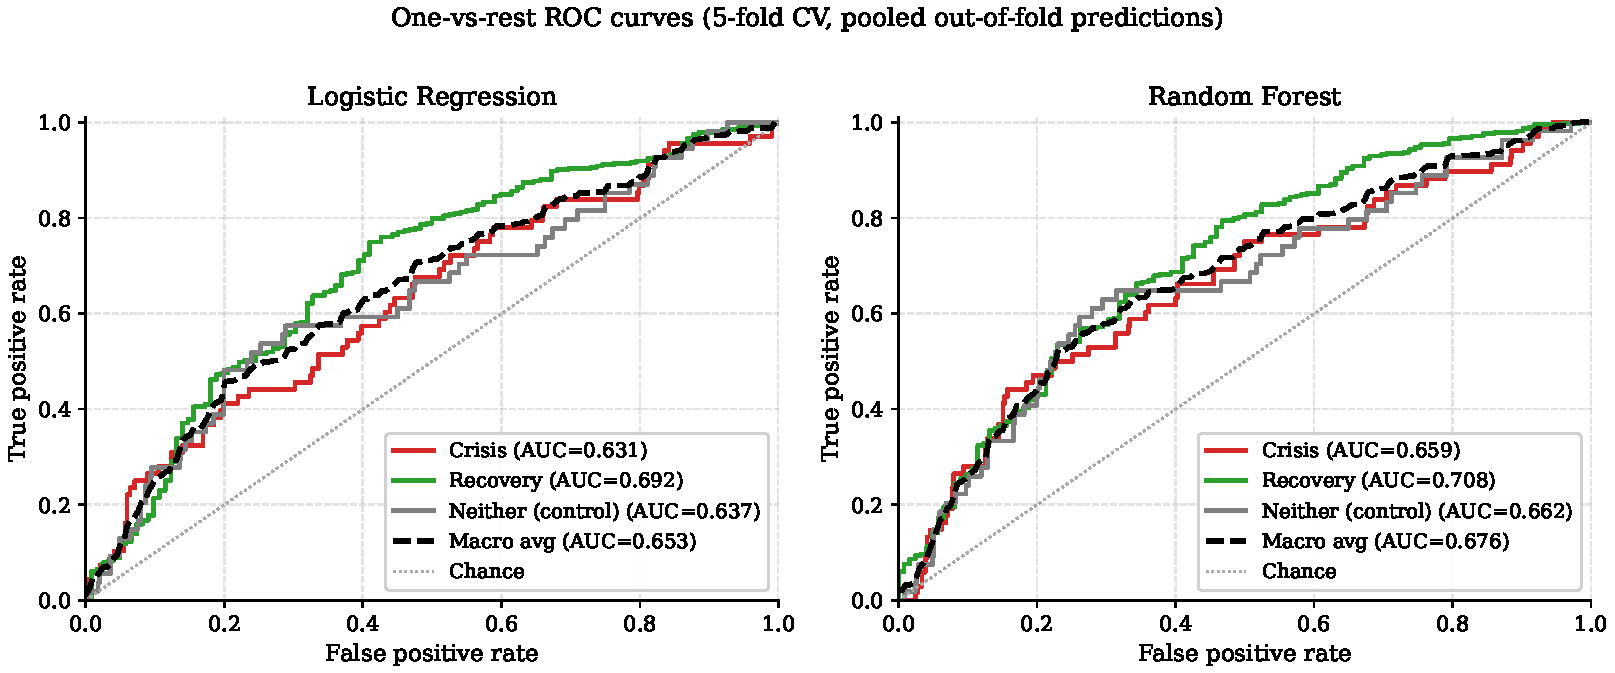
\includegraphics[width=\columnwidth]{figures/roc_curves.pdf}
  \caption{One-vs-rest ROC curves for Logistic Regression (left) and
           Random Forest (right). Dashed black line shows macro average.}
  \label{fig:roc}
\end{figure}

\subsection{Feature importance}
Figure~\ref{fig:importance} presents RF Gini importances from the
raw-feature classifier for comparability with prior work;
Section~\ref{sec:ablation} above already discusses how importance
shifts once temporal and z-norm features are added.
On raw features alone, the top-ranked features are
\texttt{ttr\_baseline} (0.055) and \texttt{sentiment\_mean\_baseline}
(0.040), followed by \texttt{sentiment\_mean\_pre\_4w} (0.036).
The dominance of \emph{baseline} features over \emph{delta} features
suggests that baseline writing style carries more classifier signal
than change from baseline---consistent with our change-vs-style
analysis in Section~\ref{sec:change-vs-style}.
When temporal features are included,
\texttt{hour\_entropy\_baseline} displaces every linguistic feature to
become the single most important predictor (Gini $\approx$ 0.054--0.060
depending on the feature set), with
\texttt{hour\_entropy\_delta\_pre\_2w} and
\texttt{late\_night\_rate\_baseline} also entering the top ten.

\begin{figure}[t]
  \centering
  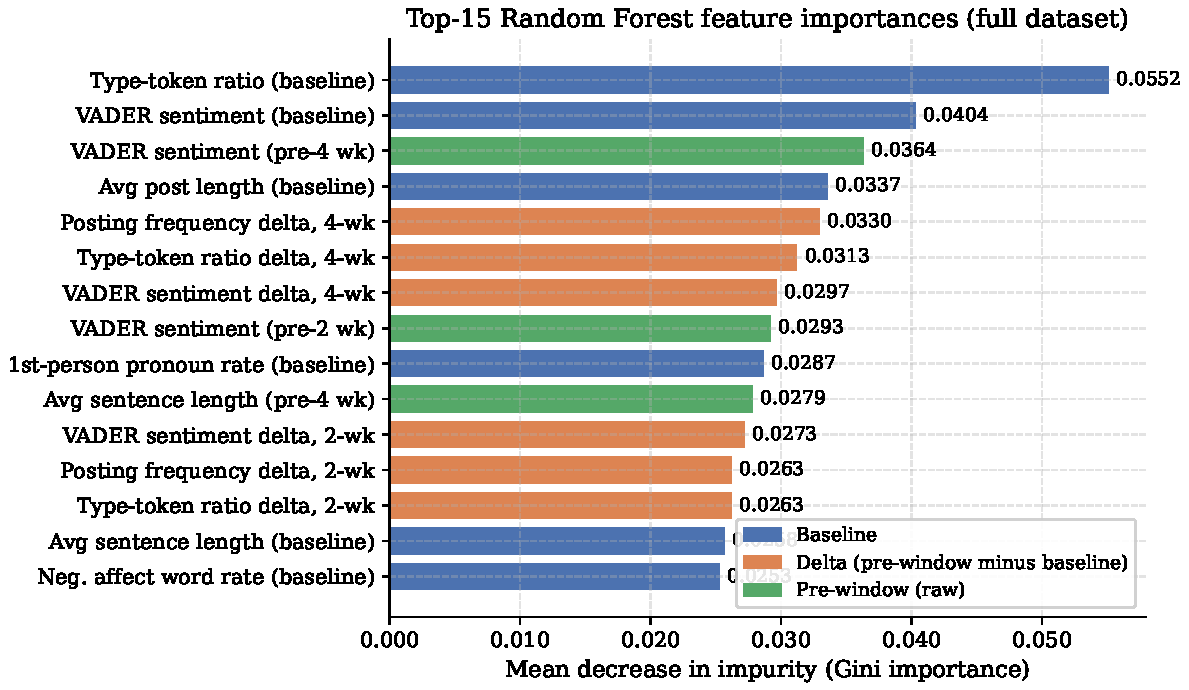
\includegraphics[width=\columnwidth]{figures/feature_importance.pdf}
  \caption{Top-15 Random Forest feature importances (full dataset).
           Blue bars: baseline features; orange: delta features;
           green: raw pre-window features.}
  \label{fig:importance}
\end{figure}

\subsection{Unsupervised change-point baseline (PELT)}
\label{sec:pelt-results}
Running PELT on weekly-mean sentiment for the 131 labelled users with
sufficient activity yields at least one detected change-point for
only $77$ of them (mean $0.98$ CPs per user).
The nearest detected change-point falls within $\pm 2$ weeks of the
ground-truth turning point for $15.3\%$ of labelled users overall
(or $26.0\%$ if we restrict to users with any detected CP), against
a random-CP null rate of $11.4\%$.
At the stricter $\pm 1$-week tolerance, PELT hits $7.6\%$ versus a
null of $5.7\%$.
The unsupervised approach is therefore only weakly above chance and
well below the supervised classifiers
(Table~\ref{tab:ablation}, macro RF AUC $\geq 0.65$).
This gap motivates the supervised feature-based framing: the pre-crisis
signal is present but not concentrated enough in univariate sentiment
alone for a purely generative change-point method to detect it.

\subsection{Sensitivity analysis}
\label{sec:sensitivity-results}
Removing the 33 low-confidence \emph{``made it''} recovery users reduces
recovery F1 from 0.139 to 0.000 (RF) and from 0.223 to 0.081 (LR),
confirming that these users contributed most of the recovery signal and
that the signal is fragile under stricter labelling.
Crisis F1 improves slightly (+0.026 RF, +0.037 LR), consistent with
label noise from miscategorised recovery users pushing some predictions
toward crisis.
Overall macro AUC drops by 0.052 (RF) and 0.029 (LR).

% ─────────────────────────────────────────────────────────────────────────────
\section{Discussion}
\label{sec:discussion}

\paragraph{What works.}
Sentiment is the most consistent signal: the $+0.22$ pre-1w recovery
delta is interpretable (people explicitly writing about feeling better)
and durable across both models.
Post frequency declines for both labelled groups before the turning point
(crisis $-0.18$ posts/week, recovery $-0.44$), suggesting that approaching
a turning point---regardless of direction---is associated with a withdrawal
from posting activity.
Sentence length diverges meaningfully: crisis users write longer sentences
($+3.0$ words) near the turning point while recovery users write shorter
ones ($-3.9$), potentially reflecting rumination vs resolution.

\paragraph{What does not work well.}
Negative-affect word rate shows almost no between-group discriminative
power; the LIWC-inspired wordlist may be too small and too literal.
First-person pronoun rate, frequently cited as a depression marker in
prior work \citep{rude2004language,coppersmith2014quantifying}, shows
only negligible differences here.
The RF's tendency to collapse predictions onto \emph{neither}---the
majority class---limits its utility for crisis detection despite its
higher ROC-AUC.

\paragraph{Generalisability.}
The cohort is small (132 labelled users) and skewed toward r/OCD
(46\% of labelled users) rather than r/depression (8\%).
Results may not transfer to other communities, languages, or time periods.
The turning-point date range (2019--2021) coincides with the COVID-19
pandemic, which may confound both baseline behaviour and turning-point
triggers.

\paragraph{Baseline style and within-user change are additive.}
The prominence of baseline TTR and sentiment in the RF importance
rankings is a cautionary finding---the classifier is partly identifying
\emph{who posts in these subreddits and how} rather than \emph{what
changes before a turning point}.
We address this directly with the per-user z-score normalisation
(Section~\ref{sec:znorm}) and deltas-only ablation, which together
show that within-user change signal exists at AUC\,$\approx$\,0.56 but
carries roughly the same information that is already present in the
raw delta columns.
The combined raw+z-norm configuration therefore performs no better
than raw alone, but the two signals are measurably independent: z-norm
post-frequency features enter the top-15 RF importance once available.
Future work should operationalise the change-vs-style distinction
directly in the objective function---for instance by training a model
that must predict label from z-normalised features alone---rather
than relying on feature importance as an indirect diagnostic.

\paragraph{Limitations.}
Four limitations bound the conclusions that can be drawn from this study.

\textbf{(1) Keyword-based label noise.}
Turning-point labels are derived from substring matching, not clinical
annotation.
False positives are inevitable: \emph{``want to die''} is used
hyperbolically; \emph{``goodbye''} may mark the end of a post, not a
person; \emph{``made it''} is unambiguously ambiguous (Section~\ref{sec:sensitivity}).
False negatives are also present---users experiencing genuine crises who
never used the listed phrases are silently assigned to \emph{neither}.
The sensitivity analysis provides a partial bound on this noise for
recovery labels, but no comparable bound exists for crisis false negatives.

\textbf{(2) OCD-dominated cohort.}
r/OCD accounts for 46\% of labelled users (61 of 132), while r/depression
contributes only 8\% (10 users).
This matters because OCD, depression, PTSD, ADHD, and autism-spectrum
conditions have distinct linguistic profiles \citep{coppersmith2014quantifying,gkotsis2016language}.
A model trained on this cohort primarily reflects the language patterns of
OCD-posting users and may generalise poorly to depression-specific
early-warning contexts---precisely the application most discussed in
prior work.

\textbf{(3) Data ends December 2021.}
The dataset spans July 2019--December 2021, entirely overlapping with the
COVID-19 pandemic.
Pandemic conditions are known to have elevated baseline anxiety, disrupted
help-seeking behaviour, and changed platform usage patterns.
We cannot disentangle longitudinal linguistic trends from period effects,
and results may not transfer to pre-pandemic or post-pandemic populations.

\textbf{(4) Baseline style dominates change signal.}
Raw baseline features rank above both delta and z-normalised features
in RF importance even when the latter are available.
Our ablation (Section~\ref{sec:ablation}) confirms that change-only
configurations reach only AUC\,$\approx$\,0.56 versus AUC\,$=$\,0.65 for
raw features.
The supervised classifier's advantage over the unsupervised PELT
baseline therefore comes partly from signal it is not the primary
claim of this paper to isolate: stable individual and subreddit style.
We report the change-only numbers directly so that the style versus
change contribution is legible to downstream readers.

\textbf{(5) Domain-general rather than mental-health-specialised
embeddings.}
The embedding features in Section~\ref{sec:embeddings} were computed
with \texttt{sentence-transformers/all-mpnet-base-v2} rather than
MentalBERT, because
\texttt{mental/mental-bert-base-uncased} and both
\texttt{mental-roberta-base} mirrors were gated repositories at the
time of writing.
Domain-specialised encoders would likely increase the incremental
contribution of the embedding features; we report our number as a
lower bound.

\paragraph{Future directions.}
Access to the MentalBERT checkpoint would let us quantify how much of
the embedding-feature shortfall is due to domain mismatch versus
information saturation of the linguistic features.
Finer temporal granularity---daily rather than weekly windows---combined
with a larger cohort would allow proper time-series modelling
\citep{yates2017depression}.
Multi-task learning across subreddits may improve generalisation,
given that r/OCD dominates the present cohort.
Finally, applying a temporally-sensitive F1 metric
\citep{tsakalidis2022identifying} that rewards predictions near but
not exactly at the turning point would let us re-score the PELT
baseline more charitably and compare it to the supervised models on
equal terms.

% ─────────────────────────────────────────────────────────────────────────────
\section{Ethics}
\label{sec:ethics}

\paragraph{Public data does not mean consequence-free data.}
The posts in this dataset were written by real individuals disclosing
genuine distress. Although Reddit content is technically public, the
authors did not consent to being included in a mental health research
dataset. We treat this asymmetry seriously.

\paragraph{Data handling.}
We do not publish raw post text, user pseudonyms, or any data that
would enable re-identification.
All released artefacts contain only aggregate statistics and derived
feature matrices.
Users in the dataset are referred to exclusively by anonymous index in any
intermediate files.

\paragraph{Keyword labelling is not clinical assessment.}
The crisis and recovery labels used here are derived from keyword
matching, not clinical diagnosis.
Phrases like \emph{``want to die''} may be used hyperbolically;
\emph{``made it''} is demonstrably ambiguous (Section~\ref{sec:sensitivity}).
These labels should \emph{never} be used to make inferences about
specific individuals' mental state.
The model outputs are correlational indicators at the population level,
not individual-level risk scores.

\paragraph{Potential for misuse.}
A model trained on this data could, in principle, be used to
surveil or profile Reddit users without their knowledge.
We strongly oppose this application.
Any deployment of similar models in a live context would require
institutional ethics approval, informed consent mechanisms, and
clinical oversight---none of which this research can provide.

\paragraph{Limitations of the research context.}
This study was conducted without access to ground-truth clinical
outcomes. We cannot verify whether a user who posted a crisis keyword
actually experienced a clinical crisis, nor whether a recovery keyword
reflected lasting recovery. All findings must be interpreted as
\emph{population-level linguistic correlates}, not causal or predictive
clinical claims.

% ─────────────────────────────────────────────────────────────────────────────
\section{Conclusion}
\label{sec:conclusion}

We presented an end-to-end pipeline for detecting longitudinal
linguistic markers of mental health turning points in Reddit data.
Our key findings are: (1) sentiment is the strongest and most
consistent single-feature signal, with a $0.29$-unit gap between
crisis and recovery users in the week before the turning point;
(2) change-only feature configurations reach macro AUC\,$\approx$\,0.56,
substantially above the $0.500$ chance level and the $0.153$
unsupervised PELT hit@$\pm 2$w baseline, but substantially below the
$0.65$ achieved by raw features that include baseline style---
quantifying how much of the total signal is due to stable individual
and subreddit style rather than pre-crisis \emph{change};
(3) adding six temporal posting-behaviour features (hour-of-day
entropy, late-night rate, etc.) yields the largest single-group lift
over raw, with hour-of-day entropy becoming the single most
important feature across every configuration that includes it;
(4) stacking linguistic, z-normalised, temporal, and embedding
features reaches macro AUC\,$=$\,$0.687$ on the three-class task
(RF, 127 features); and (5) recovery labels derived from the phrase
\emph{``made it''} are fragile---removing them drops recovery F1
by at least $0.14$.
We hope this pipeline, ablation study, and sensitivity analysis
framework will serve as a methodological building block for larger,
clinician-validated studies.

% ─────────────────────────────────────────────────────────────────────────────
\section*{Acknowledgements}
The author thanks the open-source contributors behind the
\texttt{solomonk/reddit\_mental\_health\_posts} dataset and the
Hugging Face \texttt{datasets} library.

% ─────────────────────────────────────────────────────────────────────────────
\bibliographystyle{acl_natbib}
\bibliography{references}

\end{document}
